\chapter{Software}
\label{software_chapter}

In this chapter we will describe and explain the software framework implemented to work with modular robots and test the locomotion gaits and digital hormone-based controller. This framework is named	\emph{Hormodular}, a combination of the terms ``hormone'' and ``modular''.\\

All the software developed for the \emph{Hormodular} framework is open source, and can be found in the following github repository: \url{https://github.com/David-Estevez/hormodular}. Being open source, anyone can download, use and study the code freely. This is very important in research, as any researcher interested in modular robotics in any part of the world can use this code, learn from it, improve it or repeat the experiments described in this thesis to test the validity of the results presented here.\\

This chapter will start explaining what are the software dependencies used in this project, then we will describe the Test-Driven Development methodology followed to develop the project. Next, the software structure will be discussed, with a detailed description of all the different classes implemented. Finally, the compilation procedure and program usage are offered for anyone interested on downloading and using this software.\\


\section{Software dependencies}
\label{software_dependencies}

Due to the complexity of the project, some specific tasks required the use of third-party libraries perform them. According to the open source nature of our project, these libraries were chose to be also open source, and compatible with GNU/Linux systems. These libraries are in charge of tasks such as simulation of the modular robot, optimization of the oscillator parameters in order to achieve locomotion or parsing XML configuration files.

\subsection{Simulation software: OpenRAVE}
\label{software_openRAVE}

The simulation software used by the student for this project is OpenRAVE. OpenRAVE \cite{diankov_thesis} is an Open Source project developed by Rosen Diankov that provides simulation tools for working with robots and trajectory planners. It can be embedded on other controllers and larger frameworks, and its functionality can be extended by means of plugins, adding new trajectory planners, controllers, collision checkers, inverse kinematics solvers, robots or sensors as needed.\\

OpenRAVE was chosen over other simulators due to its open source nature and its extensive documentation \cite{diankov_website:openrave}, as well as its easy integration with larger projects, such as this one.

\subsection{Modular Robotics plugin for OpenRAVE: OpenMR}
\label{software_openMR}

OpenMR \cite{gonzalez-gomez_website:openmr} is a plugin for the OpenRAVE simulator developed by Juan Gonzalez-Gomez that allows the user to simulate servo motors on the joint of OpenRAVE robots.\\

It adjusts the angular velocity of the robot joint by means of a PD controller feedbacked with the joint angular position, so that the user can control the joint position value with a simple interface.

\subsection{Evolutionary Computation Framework: ECF}
\label{software_ECF}

The Evolutionary Computation Framework (ECF) \cite{ecf:website} is a C++ library that allows the user to apply several evolutionary optimization algorithms in a very customizable way. It offers several common evolutionary optimization algorithms such as particle swarm optimization (PSO), differential evolution (DE), genetic annealing, artificial bee colony (ABC), and genetic algorithms with steady state tournament and generational roulette-wheel selection, among others.\\

By means of a XML file, the user selects the optimization algorithms to be used, and its parameters. That XML file also contains information about the genotype that will encode the different parameters to be evolved. The user can specify his own fields that can be later read by the software containing the ECF to set user-defined paramters.\\

The interface of the ECF is very simple, and to optimize a given function the user just has to inherit from the base class ``EvaluateOp'', registering the custom parameters needed by that class to be extracted from the configuration XML file, and specifying the actions to me made for the initialization and evaluation of the function with a given genotype.\\

In this case the function to be evaluated is the distance travelled by the modular robot running for a certain period of time using the oscillator parameters specified by the genotype.


\subsection{XML parsing: TinyXML2}
\label{software_tinyxml2}

TinyXML2 \cite{tinyxml2:website} is an Open Source lightweight C++ library that supports Document Object Model (DOM) parsing of XML with a very small memory footprint. DOM parsing is a cross-platform and language-independent convention for representing tagged documents such as HTML, XHTML or XML files, and means that the data inside the xml file is represented as a tree in which each node is an object that can be addressed and manipulated.\\

TinyXML2 can be easily integrated in a project with almost any configuration required. It is also has a very simple API, is fast and requires a very small amount of memory, being those the main reasons for using it in this project, instead of coding a XML parser from scratch or using a bigger XML parser.\\

XML files are used in this project for storing the robot configuration in a way that is easy for a human to setup manually, and also simple for a machine to extract that information later.\\



\subsection{Linear algebra library: Eigen}
\label{software_eigen}

Eigen \cite{eigen:website} is an Open Source C++ library for performing linear algebra operations with matrices, vectors and algorithms related to them. It is implemented as a template library that only includes header files, and supports matrices of all sizes and numeric types, including integers, floating-point numbers and complex numbers.\\

Eigen also support homogeneous transformation matrices, vector-axis pairs and quaternions, that are used in this project to obtain the relative orientation between two modules from the data obtained by the simulated IMU.\\

\subsection{Software build tool: CMake}
\label{software_cmake}

CMake \cite{cmake:website} is a cross-platform, open source build system designed to build, test and package software. Using simple and compiler-independent configuration files, CMake allows to control the build and linking process, generating all the files and environments required by the compiler chosen by the end user to build the code.\\

CMake  supports building programs that require several libraries, cross-compilation, as well as complex directory hierarchies and it is used in many large open source software projects, such as Blender, KiCAD, OpenCV, Point Cloud Library or Qt5.


\section{Development Methodology: Test-driven Development (TDD)}
\label{software_TDD}

For the development of the software of this project, the author has used a software development methodology called ``Test-driven Development (TDD)'', part of a larger set of development methods called ``Agile software development''. ``Agile software development'' methods allow a fast development of the project based on an iterative and incremental process, in which the code evolves from a simple version to the final one by adding functionality little by little as required by the project.\\

``Test-driven Development'' methodology \cite{tdd:book} is based on a short development cycle that is repeated iteratively, in which a new desired feature or improvement is used in a test case that initially fails (since there is no code for performing that feature yet). Then, the programmer implents the minimum code required to pass that test, and finally refactors the code into a clearer and more mantainable form.\\

Since every functionality in the code has a test associated, the code has a greater maintainability. Extending or improving the code becomes easier, faster and safer, since the tests can be run before commiting changes to the repository, ensuring that the new code does not break any old functionality. For example, when a team works on a software project, TDD allows them to check that the new code each member adds does not interfere with the old tested code, reducing the number of bugs and reducing the code interdependency.\\

Tests also help programmers understand the code written by other people. Since the test uses the code (functions, classes, etc) in order to test them, they can be used by programmers as a reference of how that code is supposed to be used and behave.\\

\subsection{Test-Driven Development main cycle}
\label{software_TDD_maincycle}

The main cycle of developing a new feature or improvement with a Test-Driven Development methodolody is the following:

\begin{enumerate}
	\item {\bfseries Add a test for the new feature or improvement.}\\
	When a new feature or improvement is required, a new test is written. Since there is no code yet that implement that feature, this test must fail. The test must check all the requirements of that particular feature to be added. That way, the developer can focus on the requirements and not add any unnecessary code.\\
	
	\item {\bfseries Run all tests. Check that the new one fails. }\\
	This steps checks that all previous tests pass without any issue, and that the new added test fails. The new test must fail, because there is no code yet for that feature, and that allows the developer to check whether the test was correct or not. A new test that passes without the addition of any code is useless for the programmer, since it does not check the new code to be implemented.\\
	
	\item {\bfseries Write the code for the new feature.}\\
	In this step the developer implements the minimum code required to make the test pass. This code does not need to be as eficient or elegant as the original, it just has to pass the test. This code is not definitive, and it will be improved and refined in later steps.\\
	
	\item {\bfseries Run tests.}\\
	At this point the developer has to run all the tests, including the new one. This will ensure that the code developed meets the tested requirements, and that the new code does not break any previous functionality tested in other tests.\\
	
	\item {\bfseries Refactor code.}\\
	The tested code has to be now cleaned up in order to be eficient, elegant and maintainable. In this step the code is moved to where it belongs logically within the project and encapsulated in a class if needed. If there is any duplicated piece of code, the developer should remove it, for example, by creating a function that encapsulates it. He has also to check whether the names given to functions and variables make sense and are representative of their current use. All these actions are called ``refactoring code''.\\
	
	By running againt the tests, the programmer can be confident that the refactored code still performs as required, and that the older code works as expected.\\
	
	\item {\bfseries Repeat.}\\
	Since this is an iterative process, it has to be repeated for each new feature to be added, incrementing the overall functionality of the project. These increments have to be small enough to allow a fast development and to minimize the amount of time spent in debugging the code.\\
\end{enumerate}

\subsection{Test-Driven Development example}
\label{software_TDD_example}

In order to explain better the development cycle under a ``Test-driven development'' methodology, we will present an example. In this example, we will develop a simple calculator that performs sums and wrap it on a C++ class. For the test we will use Google's GTest C++ Framework, that will be described in detail in section \ref{software_gtest}. \\

The first step is to define what is the functionality that the new code has to perform, and write the first test. In this case the functionality is to perform a simple sum, so the test will be very simple. One will usually test the error-prone or critical cases, in this case, we will test the sums of some positive numbers, the sum of positive and negative numbers, and the addition of 0. If we were developing the division function, for example, we would test the behaviour when dividing by 0, checking for example that the code raises an exception when the user tries to divide by 0.\\

The test would look like this:\\

\Cpp
\begin{lstlisting}

class TestCalculator : public testing::Test
{
	/* These class will contain the elements common to all the test, 
	but for now it is empty */
};

/* TEST_F stands for test fixture, test fixtures use a test class inheriting from testing::Test,
like TestCalculator. The first parameter is the testing::Test class to be used, and the second
one is the name of the test to be implemented. */ 
TEST_F( TestCalculator, calculatorAddsPositiveNumbers)
{
	/* EXPECT works as an ASSERT, but if the condition is not accomplished, it continues the rest
	of the test, reporting the error at the end. The expected result is placed as first argument, 
	and the expresion to be evaluated is placed as second argument.*/
	EXPECT(42, calculator.add(21, 21));
}

TEST_F( TestCalculator, calculatorAddsZero)
{
	EXPECT( 5, calculator.add(5, 0);
}

TEST_F( TestCalculator, calculatorAddsNegativeNumbers)
{
	EXPECT(-1, calculator.add(1, -2);
}
\end{lstlisting}

If we try to run this test, it will not even compile, as calculator, which is a instance of the class Calculator has not been created. In fact, the class Calculator has not been declared, so we will add it to the test, and we will instantiate it to be able to run the test:\\

\Cpp
\begin{lstlisting}
/* We add this class to the test file. Note that we did not implement the add method yet. */
class Calculator 
{
  public:
    int add( int a, int b);
};

/* We modify the test class, adding the calculator instance to be tested. */
class TestCalculator : public testing::Test
{
  public:
    Calculator calculator;
};

\end{lstlisting}

When this test is run, it should not pass any of the tests, since the functionality has not been implemented yet. Once we have checked that the test fails, we will implement the requested functionality:\\

\Cpp
\begin{lstlisting}
/* We implement the calculator class in the same file */
int Calculator::add( int a, int b)
{
    return a+b;
}
\end{lstlisting}

Running the tests now will result in all the tests passing. After this code we would refactor all the code to a more maintainable form. In case we wrote the code directly in the test, we would put it on a function or class. Since we did use a class from the beginning, refactoring will consist on moving the class to its own header file ``Calculator.hpp''. After we have refactored the code, the tests must be run again to check that the code still passes them. \\

If we want to add more features to the calculator, such as subtraction, multiplication or division, we would repeat the process again from the start, creating a new test for the new operations to be implemented.\\

\subsection{Google Test (GTest)}
\label{software_gtest}
Google Test (GTest) \cite{gtest:website} is a framework for writing tests in C++ developed used by Google in their software projects, and released publicly under a Open Source license. By means of several macros, one can add tests that are automatically discovered by GTest, as well as assertions to be ensured by the code.\\

Different tests of the same class or library can be grouped in a test fixture. As seen in the previous example (section \ref{software_TDD_example}), GTest provides a class \emph{testing::Test} that can be used to set up the data or prerequisites for the test. The programmer can define a class that inherits from \emph{testing::Test} and, before each test of the test fixture is run, the \emph{SetUp()} method implemented by the programmer will be called by GTest in order to setup the required elements used in the test. After the test is finished, the \emph{TearDown()} function will be called by GTest in order to perform the cleanup of the used elements, or to free the allocated memory.\\

Each new test is added by using the \emph{TEST()} macro, taking as argument the name of the test. If the tests are going to be grouped in a test fixture that uses the same data or instances of the class to be tested, the \emph{TEST\_F()} macro can be used instead. The \emph{TEST\_F()} macro takes two arguments: the first one is the name of the class inheriting from \emph{testing::Test} that will prepare the data for each test, and the second one is the name of the test to be implemented. GTests are recognized at compilation time, and integrated in a GTest application, that runs the tests and shows a report like the shown in figure \ref{fig:software_gtest_report}. \\

\begin{figure}[h]
		\centering
        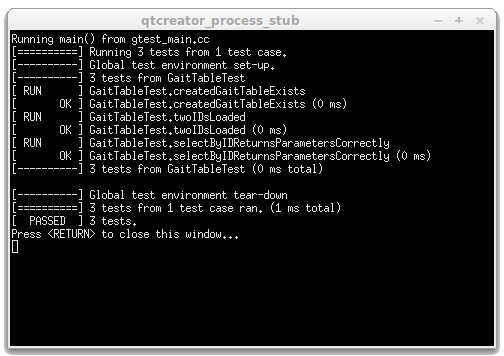
\includegraphics[width=0.6\textwidth]{images/software_gtest_report.png}
        \caption{GTest report}\label{fig:software_gtest_report}
\end{figure}

Inside the test, the conditions that have to be ensured are checked with the macros \emph{ASSERT()} and \emph{EXPECT()}. The main difference between them is that if \emph{ASSERT()} is used, the execution of the test ends if the condition imposed is not met, whereas if \emph{EXPECT()} is used instead, the execution of the test continues even thought that condition fails. One typically uses \emph{ASSERT()} when the test cannot continue if the condition fails, or if it has no sense to continue with the test if the condition fails. On the other hand, using \emph{EXPECT()} allows the program to continue testing the code, so that if more than one bugs are present they can be found on the same run of the test, and corrected at the same time, speeding up the debugging process.\\

\subsection{Hormodular tests}
\label{software_testexplanation}
To develop the software of this project a test-driven development was followed, and several tests were consecutively implemented, increasing the project functionality until the project was completed. Here were will describe what functionality is tested on each of the tests.

\begin{itemize}
	\item \textbf{TestConfigParser}: Tests that the class \emph{ConfigParser} is able to parse a test configuration file and extract from it the configuration parameters.
	
	\item \textbf{TestConnectionsFromConfigParser}: Tests the module interconnection. It creates a series of modules and attaches them according to the information stored in a \emph{ConfigParser}, checking the connections. After that, runs the hormone communication protocol and tests that the IDs calculated by the hormones are the correct ones.
	
	\item \textbf{TestGaitTable}: Tests the main functionality of a gait table: loading the data from a text file and returning the parameters stored correctly.
	
	\item \textbf{TestModularRobot}: Creates a \emph{ModularRobot} with a \emph{SimulatedModularRobotInterface} and tests that the \emph{ModularRobot} is able to move at least 10cm in 25ms.
	
	\item \textbf{TestMovement}: Creates a series of \emph{SinusoidalOscillators} with the parameters required for a 2-module snake robot to move in straight line ($A = 60º$, $O = 0º$, $\Delta\phi = 120º$, $T = 1s$) and sends the joint position to the simulated module using a \emph{SimulatedModularRobotInterface}, testing that the snake robot moves more than 10cm.
	
	\item \textbf{TestMovementWithGaitTable}: Similar to the previous test, but in this case the parameters are loaded on a \emph{GaitTable} from a file, and later retrieved from the \emph{GaitTable} and set on the \emph{SinusoidalOscillator}.
	
	\item \textbf{TesOrientation}: Tests the different mathematical operations that can be performed with the \emph{Orientation} class, such as sums and substractions. It also tests that the calculation of the relative orientation between two connectors is performed correctly.	
	
	\item \textbf{TestSerialCommSinusoidal}: Tests the connection with the robot by opening a serial port and sending to the robot joint values that follow a sinewave.
	
	\item \textbf{TestSerialModularRobotInterface}: Tests that the modular robot joints move when the joint values are sent with the \emph{SerialModularRobotInterface}. It also tests toggling the LED on the controller board.

	\item \textbf{TestSimulatedModularRobotInterface}: Tests that the simulated robot joints move when the joint values are sent with the \emph{SimulatedModularRobotInterface}.
		
	\item \textbf{TestSinusoidalOscillator}: Tests that the \emph{SinusoidalOscillator} outputs values according to a sine function.
	
\end{itemize}

\section{Software structure}
\label{software_structured}

The software was developed with modularity and code reusability in mind, defining several interfaces that help to add new features or implement the existing ones in a different way. The main class of the project is the \emph{ModularRobot} class, that represents a modular robot made of a series of modules. With this class is possible to test different controllers for the modules, use different kinds of oscillators to generate the locomotion gaits or interface with different modular robots (both simulated and real). In this section the general structure of the code will be explained, including a detailed description of each of the different classes that compose the \emph{ModularRobot} class, and their function in the project.\\


The class \emph{ModularRobot} models the whole modular robot as a set of \emph{Modules}. Even thought the controller is distributed in nature, the hardware used to test the gaits is centralized, having only a single controller board, so this class is needed to join the distributed controllers into a single robot encapsulating them in order to communicate with the hardware. The \emph{ModularRobot} is configured using a xml file read by the \emph{ConfigParser}, which uses the TinyXML2 library to load the configuration parameters in the xml file to a data structure that the \emph{ModularRobot} and the \emph{Module} can access for setting their parameters.\\

\begin{figure}[h]
		\centering
        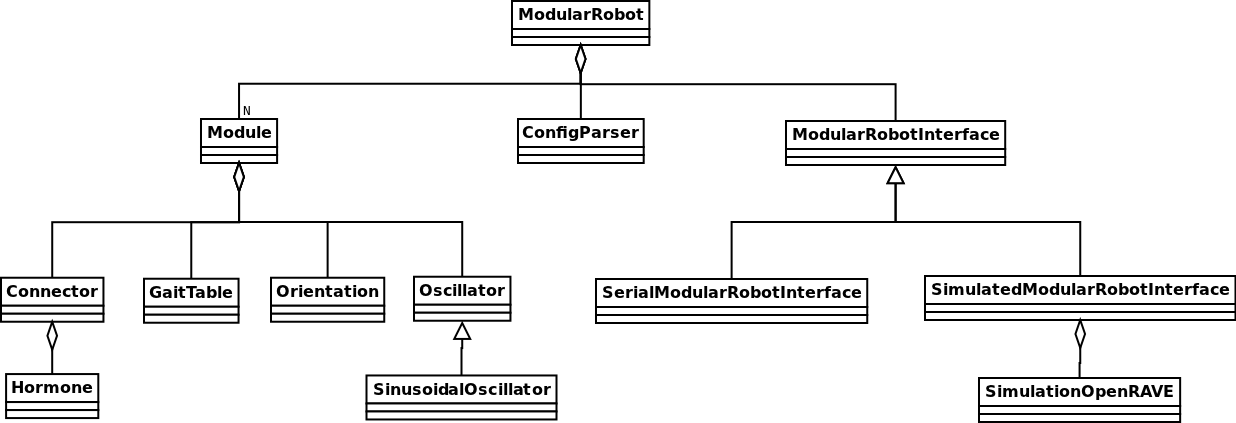
\includegraphics[width=\textwidth]{images/Class_diagram_Main.png}
        \caption{Main class diagram}\label{fig:software_class_main_class}
\end{figure}


Each \emph{Module} has several \emph{GaitTables} to store the parameters of the \emph{SinusoidalOscillator} for the different configurations. At each step of the controller, the \emph{SinusoidalOscillator} class calculates the joint position according to the oscillation. The \emph{SinusoidalOscillator} can be changed by another kind of oscillator thanks to the \emph{Oscillator} interface. The joint angle calculated the \emph{Oscillator} in each \emph{Module} is sent to the robot using a \emph{ModularRobotInterface} interface. \emph{ModularRobotInterface} offers a interface so that several types of robots can be used, either simulated (using the \emph{SimulatedModularRobotInterface}) or real robots communicated through a serial connection (using the \emph{SerialModularRobotInterface}).\\

A \emph{Hormone} class was defined in order to implement the hormone-communication protocol. \emph{Hormones} are sent and received by the any of the four \emph{Connectors} present in each \emph{Module} that model the interconnection of the different modules, allowing the \emph{Hormones} to flow through the modular robot.\\

Finally, the \emph{Orientation} class is a data structure for storing the Tail-Bryan angles (Roll, pitch and yaw) that are obtained by the simulated Inertial Measurement Unit. 


%%%%%%%%%%%%%%%%%% ModularRobot %%%%%%%%%%%%%%%%%%%%%%%%%%%%%%%%%%%%%%%%%%%%%%%%%%%%%%%%%%%%%%%%%%%%%%%%%%%%%%
\subsection{Class ModularRobot}
\label{software_class_modularrobot}

\begin{figure}[h]
		\centering
        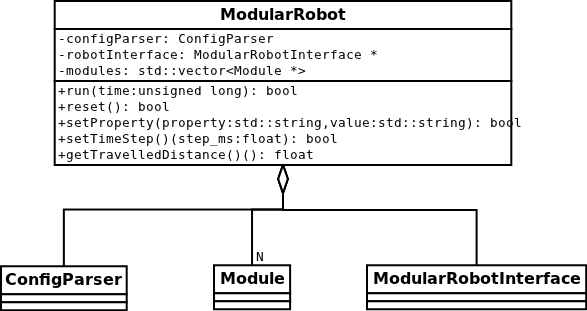
\includegraphics[width=0.6\textwidth]{images/Class_diagram_ModularRobot.png}
        \caption{ModularRobot class diagram}\label{fig:software_class_modularrobot_class}
\end{figure}


\emph{ModularRobot} is the class that encapsulates both the modules and interface with the actual robot (either simulated or real). It counts with several functions that control the robot to perform several operations such as starting or resetting the controllers of all the modules, etc.\\

A \emph{ModularRobot} is constructed using a \emph{ConfigParser} containing the configuration of the modular robot, read from a xml configuration file, which determines the number of modules to be created. A suitable \emph{ModularRobotInterface} is also created, depending on if the robot to be controlled is a real one or a simulation of the modular robot.\\

A series of functions exist to configure the behavior of the \emph{ModularRobot} after the object is created.  The function \emph{setTimeStep()} configures the resolution of the simulation for the simulated robot and the period between packet transmission for the robot controlled by serial port, and using \emph{setProperty()} one can configure other aspects such as enabling/disabling the simulation viewer.\\

After the robot parameters are configured, the module interconnections are read from the \emph{ConfigParser}, and the connectors of the different modules are connected together according to that configuration. This interconnection allows the communication of the different hormones between the modules.\\

Once the robot is configured, and its modules are connected, to start it, the function \emph{run()} is called passing the amount of time, in ms, that the robot will be active. After that amount of time the robot will stop until it receives another call to the \emph{run()} method. Before running again the robot controller, is recommended to make a call to the function \emph{reset()}, to restore the initial configuration, position of the simulated robot, etc.\\

Even though the controller is distributed, and it is supposed to be run in each of the modules independently, the current implementation is simplified to a sequential execution in order to test the hormone-communication protocol in a quick way, so that it can be validated or discarded on an early development stage. Concurrent software is typically difficult to develop and debug, since resources are shared between processes/threads and bugs may appear depending on the order in which those resources where accessed, which causes the appearance of bugs that are difficult of reproduce and fix, since that order is not deterministic. Other common bugs in concurrent software are corruption of data due to simultaneous access to unprotected shared variables or deadlocks ( a process $p_1$ has a lock $l_1$ and it is waiting for another lock, $l_2$, which is held by a process $p_2$ which happens to be waiting for the lock $l_1$).\\

Because of those reasons, the different tasks to be performed by the module controller are implemented as independent member functions, and they are called sequentially for every module before executing the next one. This way a performance similar to the concurrent approach is achieved, but without the increase in development difficulty and time due to concurrent programming. Communications tasks are executed each $T_{comm}$ ms, whereas the joint position is updated each $T_{step}$ ms, allowing to update the joint values more frequently, as the communication tasks can be performed with a larger period, since it is not a time-critical task.\\

Figure \ref{fig:software_class_modularrobot_flowchart} shows the flowchart of the \emph{run()} function of class \emph{ModularRobot}.\\

\begin{figure}[h]
		\centering
        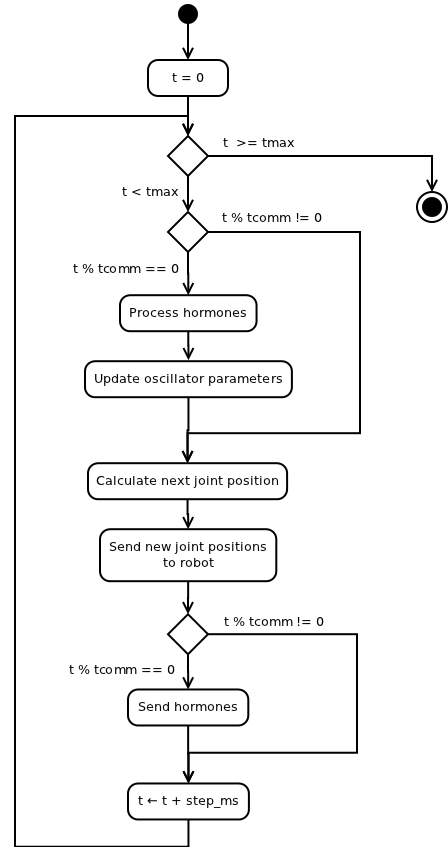
\includegraphics[width=0.4\textwidth]{images/Flowchart_ModularRobot_run.png}
        \caption{ModularRobot::run() flowchart}\label{fig:software_class_modularrobot_flowchart}
\end{figure}

The whole function runs in a loop, repeated until the maximum runtime, $t_{max}$, is reached. Each $t_{comm}$ ms the hormone functions are executed. These functions process the input hormones, obtaining the identifiers for the current module's position, function and global configuration, and setting the required hormones in the output buffers, ready to be sent to the other modules. After the different IDs have been calculated, the oscillator parameters are obtained from the gait tables and set.\\

The next steps, that are executed every $t_{step}$ ms, are the joint values updates. First, the \emph{Oscillator} calculates the new joint value for all the joints at the current time $t$ and, after that, those values are sent to the robot (simulated or real) using the \emph{ModularRobotInterface}.\\

Finally, also each $t_{comm}$ ms, the hormones that were placed on the output buffers are actually sent to the other modules. The time counter is incremented and the loop repeats again until $t_{max}$ seconds have passed.\\

It is important to notice that each of these tasks are executed for each of the modules on the modular robot before moving on to the next task, emulating this way a distributed, concurrent system.\\ 


%%%%%%%%%%%%%%%%%% ConfigParser %%%%%%%%%%%%%%%%%%%%%%%%%%%%%%%%%%%%%%%%%%%%%%%%%%%%%%%%%%%%%%%%%%%%%%%%%%%%%%
\subsection{Class ConfigParser}
\label{software_class_configparser}


\begin{figure}[h]
		\centering
        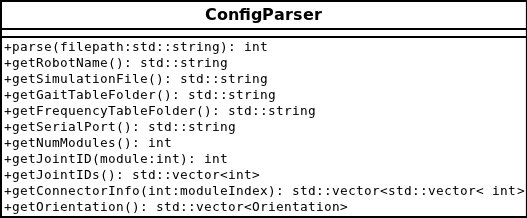
\includegraphics[width=0.6\textwidth]{images/Class_diagram_ConfigParser_members.png}
        \caption{ConfigParser class diagram}\label{fig:software_class_configparser_class}
\end{figure}

Since the \emph{ModularRobot} can be executed with different configurations, it is very convenient to have a way to load those different configurations dynamically without recompiling the whole software. The approach typically followed to achieve this is to use configuration files specifying the different aspects to be configured.\\

For the configuration files, the xml format was chosen, because it is standard, can be read and edited easily by both humans and machines, and there already exist several libraries for parsing xml from different programming languages.\\

The \emph{ConfigParser} class uses one of those libraries, called ``TinyXML2'' to parse the configuration files for the different robot topologies and stores the different parameters loaded in a data structure that can be later accessed by the other components of the project.\\

The tag structure of the configuration files is the following:

\begin{itemize}
	\item All the xml tags of the robot are enclosed on a parent tag called \emph{<ModularRobot>}. This tag has an atribute \emph{``name''} that contains the name of the robot.
\XML
\begin{lstlisting}
<ModularRobot name="TestRobot">
	
    <!-- Robot config goes here -->
	
</ModularRobot>
\end{lstlisting}
	
	\item Inside \emph{<ModularRobot>} go the global configuration parameters and the definition of the different modules. The global parameters to be configured are: the path to the openRAVE xml model of the robot for the simulation, with the tag \emph{<simulationFile>}; the path to the folder containing the gait tables, with the tag \emph{<gaitTableFolder>} and the path to the file with the table containing the frequencies of the oscillators for the different configurations, \emph{<frequencyTable>}. The serial port used to communicate with the real robot is configured in the tag \emph{<serialPort>}.
	
\newpage
\XML
\begin{lstlisting}
<ModularRobot name="TestRobot">

    <simulationFile>../../data/models/REPY-2.1/MultiDof-7-tripod.env.xml</simulationFile>
    <gaitTableFolder>../../data/gait tables/</gaitTableFolder>
    <frequencyTable>../../data/gait tables/frequencies.txt</frequencyTable>
    <serialPort>/dev/ttyUSB0</serialPort>
	
    <!-- Rest of the configuration goes here -->
	
</ModularRobot>
\end{lstlisting}
	
	\item Modules are defined after that, using the tag \emph{<Module>}. Inside this tag, the different parameters of the module are to be set, such as the joint index ( set with \emph{<Joint>}), the initial orientation of the module and the different connections between modules.
	
	The initial orientation defined in the configuration file under the tag \emph{<Orientation>}  is the one the module takes as if it were the readings of the Inertial Measurement Unit, emulating this piece of hardware that the current module version lacks. The different values for the angles are set in the tags \emph{<Roll>}, \emph{<Pitch>} and \emph{<Yaw>}, respectively.\\
	
	Connections between modules are set under the tag \emph{<Connections>}. Each of the local connectors (front, right, back and left) has its own tag for setting the parameters of that connector. Those parameters are atributes of the corresponding tag, such as \emph{connectedTo}, indicating which module is the current connector connected to; \emph{connector}, which represents the index of the remote connector that is connected to the current connector (0 for front, 1 for right, 2 for back and 3 for left) and  \emph{orientation}, which represents the relative orientation of the connectors, and that currently it is only used for debugging and testing purposes.

	Here we have an example of a complete xml robot configuration file for a simple 2-module configuration:
	\XML
\begin{lstlisting}
<ModularRobot name="TestRobot">
    <simulationFile>../../data/models/REPY-2.1/Kusanagi-2.env.xml</simulationFile>
    <gaitTableFolder>../../data/gait tables/</gaitTableFolder>
    <frequencyTable>../../data/gait tables/frequencies.txt</frequencyTable>
    <serialPort>/dev/ttyUSB0</serialPort>  	
    <Module>
        <Joint>0</Joint>		
        <Connections>
            <front connectedTo="1" connector="Back" orientation="0"></front>
        </Connections>
        <Orientation>
            <Roll>0</Roll>
            <Pitch>0</Pitch>
            <Yaw>0</Yaw>
        </Orientation>
    </Module>
    <Module>
        <Joint>1</Joint>
        <Connections>
           <back connectedTo="0" connector="Front" orientation="0"></back>
         </Connections>
        <Orientation>
           <Roll>0</Roll>
           <Pitch>0</Pitch>
           <Yaw>0</Yaw>
        </Orientation>
    <Module>
</ModularRobot>
\end{lstlisting}
	
\end{itemize}

\newpage

%%%%%%%%%%%%%%%%%% ModularRobotInterface %%%%%%%%%%%%%%%%%%%%%%%%%%%%%%%%%%%%%%%%%%%%%%%%%%%%%%%%%%%%%%%%%%%%
\subsection{Class ModularRobotInterface}
\label{software_class_modularrobotinterface}

\begin{figure}[h]
		\centering
        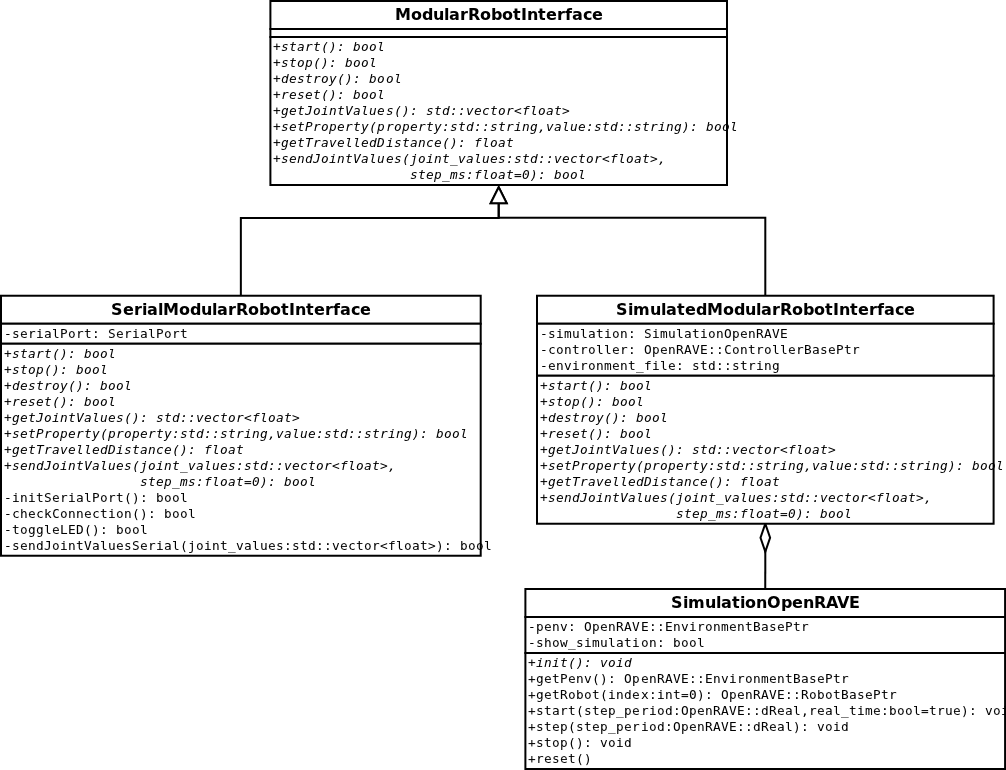
\includegraphics[width=0.9\textwidth]{images/Class_diagram_ModularRobotInterface.png}
        \caption{ModularRobotInterface class diagram}\label{fig:software_class_modularorobotinterface_class}
\end{figure}

Although the controller is distributed, the modular robot used to test the gait has a central controller, due to hardware limitations of the modules used in this work. For that reason, the \emph{ModularRobot} class owns a interface with the modular robot, in order to send commands to it, so that it can set the joints of the robot to the desired values or, in the future, receive sensor data from the robot, to implement more complex controllers.\\

The class \emph{ModularRobotInterface} acts as a bridge between the controller, being run on the computer, and the robot. As the robot to be controlled can be either a simulated one, for gait discovery and testing or the physical one, to verify that the gaits work on the real worl, this class is an abstact class that act defining the interface in a computer science sense, that is, the functions that the classes that follow this interface must define. This way, the different interfaces for the different types of robot can be used indistinctly by the modular robot controller, just having to change which class is instantiated to change the behaviour of the program.\\

Two different classes have been implemented following the \emph{``ModularRobotInterface''} ~interface:
\begin{itemize}
	\item \emph{SimulatedModularRobotInterface}, to control the modular robot simulated on openRAVE.
	\item \emph{SerialModularRobotInterface}, that controls the physical robot via the  computer serial port.
\end{itemize}
Instances of those clases are created using a factory method pattern, a function that generates objects that follow a certain interface without needing to specify the exact class of object that will be created.\\

The interface has four main functions to implement for the initialization and destruction of the interface, one for the setup of certain properties or variables, and three for the control of the robot. The purpose of each of the function is the following:

\begin{itemize}
	\item bool \emph{start()}: this function is used for the initialization of the robot interface, for example, to start the simulation or to connect to the robot with the serial port.
	
	\item bool \emph{stop()}: with this funtion the robot interface is stopped. This can be used, for instance, to stop the simulation or to interrupt the communication via serial port.
	
	\item bool \emph{destroy()}: this function is meant to be called in order to free all the dynamically allocated memory and to do all the required steps in order to destroy the object.
	
	\item bool \emph{reset()}: used to reset the interface, for example, restarting the simulation or the serial connection.
	
	\item bool \emph{setProperty(} std::string property, std::string value\emph{)}: this function should be used to configure the different properties or parameters of the interface. The string property specifies which is the property to modify, and the string value contains the new value for that parameter. This can be used, for example, to specify if the simulator viewer is to be visible or not.
	
	\item bool \emph{getTravelledDistance()}: returns the distance travelled by the robot. The method used for calculating this distance depends on the implementation of the robot interface.
	
	\item bool \emph{sendJointValues(} std::vector<float> joint\_values, float step\_ms = 0\emph{)}: sends the desired joint values to the robot. The step\_ms parameter can be used to specify the amount of time to wait for the joints to reach the position, in order to run the simulation for the time of that step, for example.
	
	\item std::vector<float> \emph{getJointValues()}: returns all the joint positions stored in a vector.
\end{itemize}

%%%%%%%%%%%%%%%%% SIMULATED ROBOT INTERFACE %%%%%%%%%%%%%%%%%%%%%%
\subsection{Class SimulatedModularRobotInterface}
\label{software_class_simulatedmodularrobotinterface}

This class implements the \emph{ModularRobotInterface} interface, and it is used to start a simulation and control the simulated robot. For that purpose it uses a \emph{SimulationOpenRAVE} objects that encapsulates all the details of starting a OpenRAVE simulation and controlling it. \\

If the simulation is to be run continously, it can be started with the \emph{start()} function. If not, the simulation is run step by step, with the step time specified in the \emph{sendJointValues()} method. The \emph{stop()} and \emph{reset()} methods stop and restart the OpenRAVE simulation and with the \emph{destroy()} method the memory for the simulation object can be freed.\\

The user can decide whether or not the simulation viewer is enabled by calling the \emph{setProperty()} method with the property ``viewer'' and the value ``enabled''.\\

For the travelled distance calculation, the initial position of the robot is stored at the start of the simulation, and when the function \emph{getTravelledDistance()} is called, that distance is calculated by computing the distance between that initial point and the current position. Calculated this way, the distance is always less than actual distance travelled, unless the robot moves in a straight line, which favors that the gaits resulting from the evolutionary algorithm follow a straight line, as this way the fitness value (average speed) is greater. \\

The joint values are accessed directly through a reference to the OpenRAVE Controller that is set on the robot, both for sending the new joint values, or to read the current ones. A step time can be specified, so that the simulation is advanced that amount of time for the joints to have time to move to their desired positions.\\

%%%%%%%%%%%%%%%%% SIMULATION OPENRAVE %%%%%%%%%%%%%%%%%%%%%%%%%%%%%%
\subsection{Class SimulationOpenRAVE}
\label{software_class_SimulationOpenRAVE}

In this work, OpenRAVE has been chosen as simulator, but many others exist. Having a class for encapsulating the simulation allows not only to add support to different simulators in the future, but also to offer a simple and generic interface for interacting with the simulation.\\

The \emph{SimulationOpenRAVE} class offers a control interface similar to the \emph{ModularRobotInterface} one, with functions for starting, stopping and resetting the simulation. It has also a function \emph{step()} to run the simulation step by step, instead of running it continuously.\\

It creates a OpenRAVE simulation, loads the environment with the modular robot to be simulated, sets the Servocontroller from the OpenMR plugin for controlling all the joints, gets references to the environment and robots, which can be later obtain with the \emph{getPenv()} and \emph{getRobot()} methods.\\

The viewer offered by OpenRAVE can be enabled either when creating the \emph{SimulationOpenRAVE} object or later, calling the \emph{showViewer()} method.\\

%%%%%%%%%%%%%%%%% SERIAL ROBOT INTERFACE %%%%%%%%%%%%%%%%%%%%%%
\subsubsection{Class SerialModularRobotInterface}
\label{software_class_serialmodularrobotinterface}

The \emph{SerialModularRobotInferface} class implements the \emph{ModularRobotInterface}, and it is used to send the joint values to the real robot through a serial connection.\\

When the \emph{start()} method is called, the serial port is open and the program connects with the modular robot until the communication is interrupted by calling \emph{stop()} or \emph{reset()}. Once the communication is halted, the allocated memory can be freed by calling the \emph{destroy()} method.\\

The joint values are sent to the robot using the function \emph{sendJointValues()}, which internally converts the values from the range of the oscillator ($[-90,90]$) to the range of the hardware servos ($[0,180]$) before sending them through the serial port. Since the robot does not count with any means of measuring the actual joint position, the sent values are stored in the \emph{SerialModularRobotInferface}, and can be requested by the user calling the \emph{getJointValues()} method.\\

Since the modular robot currently cannot sense its actual position (using internal measurements or with computer vision employing an external camera), the \emph{getTravelledDistance()} method just outputs a warning explaining that the distance travelled measurement is not implemented yet.\\

Finally, since the controller board has a LED available for visual signaling, a property called ``LED'' with a value ``toggle'' can be set to the \emph{SerialModularRobotInferface} using the \emph{setProperty()} method to turn it on and off.\\


%%%%%%%%%%%%%%%%%% Module %%%%%%%%%%%%%%%%%%%%%%%%%%%%%%%%%%%%%%%%%%%%%%%%%%%%%%%%%%%%%%%%%%%%
\subsection{Class Module}
\label{software_class_module}

\begin{figure}[h]
		\centering
        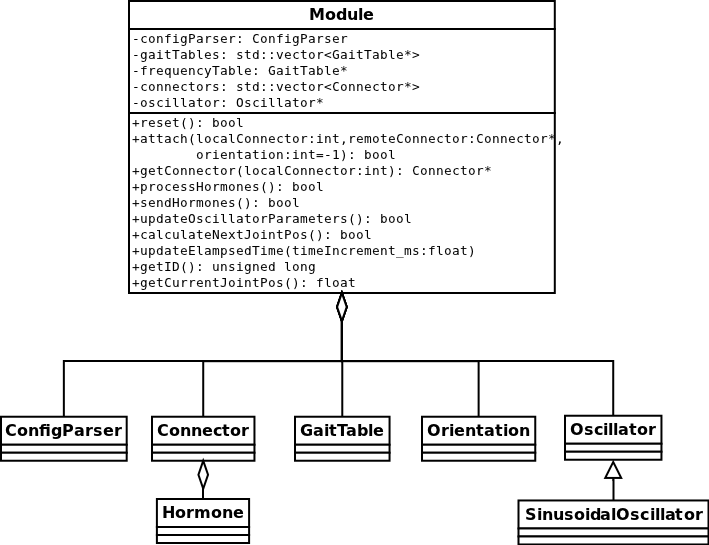
\includegraphics[width=0.6\textwidth]{images/Class_diagram_Module.png}
        \caption{Module class diagram}\label{fig:software_class_module_class}
\end{figure}

The class \emph{Module} represents the controller of each of the modules. This controller is homogeneous for the whole modular robot, each module is an instance of the same Module class.\\

A \emph{ConfigParser} is passed to the constructor with the parameters read from the configuration file, as well as the index of the module to be created, so that the correct parameters are extracted from the \emph{ConfigParser}.\\

For generating the oscillations, the \emph{Module} class has a \emph{Oscillator} object, that updates the joint position of the module. For this thesis the oscillators used are \emph{SinusoidalOscillator}, but as the \emph{Oscillator} class defines a interface for oscillators, new kinds of different oscillators can be added very easily to the project, and used without changing the code for the \emph{Module} controller.\\

The parameters for the oscillator are stored on several \emph{GaitTables}, one for the main parameters (amplitude, offset and phase) for each of the three configurations discussed on this work, and a extra one for the different frequencies for each configuration. These parameters are accessed using the IDs obtained through the hormone communication protocol. How to calculate those IDs is explained on section \ref{config_repy_description}, and the hormone communication protocol is presented on chapter \ref{hormones}.\\

One of the required data for calculating the IDs is the initial orientation of the module. There exists a class in this project, called \emph{Orientation}, that stores the data for the orientation angles. It has also several functions to do simple operations with \emph{Orientations}, as well as a function that calculates the relative orientation between the orientations of two modules, a piece of data that is key to the ID calculation.\\

For the interconnection of modules, and their communication, a class \emph{Connector} was implemented. There are 4 connectors on each module, and each \emph{Connector} has an input buffer and an output buffer to store the incoming and outgoing \emph{Hormones}, and a reference pointing to the remote \emph{Connector} they are attached to. The \emph{Hormone} class models the different types of hormones used in the hormone communication protocol, to be explained in chapter \ref{hormones}.\\ 

In order to emulate the distributed controller from a sequential approach, so that the software can be developed and validated in a faster way, the controller of the module is split in several small tasks, that are executed for all the modules before starting the next one.\\

The first task to be executed is the hormone processing. Hormones are recovered from the connectors' input buffers and processed depending on their type, as explained in section \ref{hormone_algorithm}. ``Ping'' hormones are processed first, obtaining from them the ID related to the position of the module inside the modular robot.  Then, the ``Leg'' hormones are either processed or generated in case of the ``leg'' modules. From the ``Leg'' hormones the ``head'' module will discover which is the global configuration of the robot and will generate ``Head'' hormones. Finally, if the module is not the ``head'' module,  those ``Head'' hormones are processed, obtaining the configuration ID obtained by the ``head'' module. Generated hormones are put in the output buffer in this task, ready to be sent to the connected modules.\\

Once the IDs are obtained, the next task to be performed consists in querying the new oscillator parameters to the corresponding gait tables, and setting them on the oscillator. With the ID of the current configuration the corresponding gait table for the amplitude, offset and phase of the oscillators is selected, and using the ID related to the function inside the modular robot global configuration the suitable parameters are obtained from the table and set on the oscillator. This task, as well as the previous one, are executed periodically at a different rate than the joint position update, with a period of $t_{comm}$ milliseconds.\\

After that, the oscillator will update the joint value for the module, calling \emph{calculateNextJoinPos()} with the elapsed time as parameter. The modular robot will recover this joint position value, put it in a vector with the other modules' joint values and send them to the \emph{ModularRobotInterface}.\\

Finally, the hormones stored in the output buffers will be sent to their destination modules, and the local elapsed time of the module will be updated.\\


%%%%%%%%%%%%%%% Oscillator %%%%%%%%%%%%%%%%%%%%%%%%%%%%%%%%%%%%%%%%%
\subsection{Class Oscillator}
\label{software_class_oscillator}

In order to generate the oscillations that drive the joints of the modular robot in order to achieve locomotion, the \emph{Oscillator} class is employed. This class is designed as an abstract class that stores the main oscillator parameters, and lefts the actual implementation of the oscillator to the classes that implement this interface. This way, the module controller can work with several types of oscillators without changing the controller code, just switching the \emph{Oscillator} class used.\\

The calculation of the joint position from the elapsed time is performed on the function \emph{calculatePos()}, which has to be implemented in the classes that follow the \emph{Oscillator} interface.\\
\begin{figure}[h]
		\centering
        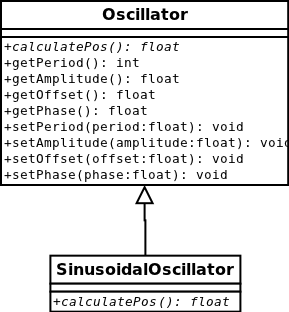
\includegraphics[width=0.3\textwidth]{images/Class_diagram_Oscillator.png}
        \caption{Oscillator class diagram}\label{fig:software_class_oscillator_class}
\end{figure}


\subsection{Class SinusoidalOscillator}
\label{software_class_sinusoidaloscillator}

The only type of \emph{Oscillator} implemented in this project is the \emph{SinusoidalOscillator}, which models the joint position values as an oscillating sinewave.\\

The \emph{calculatePos()} method calculates the position following a sinusoidal function, characterized by the amplitude, offset, phase and period stored on the \emph{Oscillator} base class. Using the elapsed time, the joint position is calculated the following way:
\begin{equation} \label{eq:software_sinusoidal_oscillator}
\varphi(t) = A_i \cdot \sin{\left( \frac{2\pi}{T} \cdot t + \Phi_i \right)} + O_i
\end{equation}\\

Sinusoidal oscillators are explained in more detail on section \ref{gait_sin_osc}.

%%%%%%%%%%%%%%% Connector   %%%%%%%%%%%%%%%%%%%%%%%%%%%%%%%%%%%%%%%%%
\subsection{Class Connector}
\label{software_class_connector}

\begin{figure}[h]
		\centering
        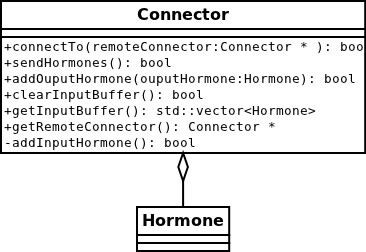
\includegraphics[width=0.3\textwidth]{images/Class_diagram_Connector.png}
        \caption{Connector class diagram}\label{fig:software_class_connector_class}
\end{figure}


In order to model the different connectors that allow the modules to be attached to other modules, the \emph{Connector} class is used.\\

The \emph{Connector} class is a simple data container that has two buffers, one for storing the incoming hormones prior to their processing, and other for placing the outgoing hormones before they are actually sent to the remote connector attached to this connector.\\

This class also contains a reference to the remote \emph{Connector} attached to this connector, in order to be able to send the hormones from the ouput buffer. This reference is set with the \emph{connectTo()} method.\\

For sending out the hormones in the output buffer to the remote module input buffer, the method \emph{sendHormones()} is used, which takes the hormones stored in the ouput buffer and puts them in the input buffer of the remote module using the reference to that module and the \emph{addInputHormone()} function.\\

The \emph{localOrientation} attribute contains the relative orientation between the local and remote modules calculated by hand. This attribute is no longer in use by the controller, which currently calculates it from the orientation of both modules, dynamically.\\


\subsection{Class Hormone}
\label{software_class_hormone}

\begin{figure}[h]
		\centering
        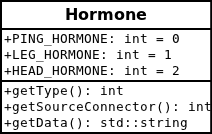
\includegraphics[width=0.2\textwidth]{images/Class_diagram_Hormone_members.png}
        \caption{Hormone class diagram}\label{fig:software_class_hormone_class}
\end{figure}

The \emph{Hormone} class is the base for the hormone communication protocol, one of the key aspects of this work. The class is a container for the info that is needed to be transmitted to the other modules.\\

A \emph{Hormone} has 3 fields: the type of hormone (``Ping'', ``Leg'' or  ``Head''), encoded as an integer; the connector that sent the hormone, also encoded as integer (0, 1, 2 and 3 for the front, right, back and left connectors, respectively) and a data field to attach extra info required for the modules to discover the IDs.\\

The contents of the data field depend on the type of hormone. ``Ping'' hormones store in the data field the local orientation of the module that sends the hormone as a string (i.e. ``90 180 270'', meaning roll=90º, pitch=180º and yaw=270º). ``Leg'' hormones do not need any extra info, so their data field is empty, and ``Head'' hormones store in the data field the ID of the global configuration as discovered by the ``head'' module ( 0 for \emph{MultiDof-11-2}, 1 for \emph{MultiDof-7-tripod} or 2 for  \emph{MultiDof-9-quad}) and, if needed, an extra integer for leg dissambiguation.\\

The hormone communication protocol is explained in detail on chapter \ref{hormones}.\\

\newpage

\subsection{Class GaitTable}
\label{software_class_gaittable}

\begin{figure}[h]
		\centering
        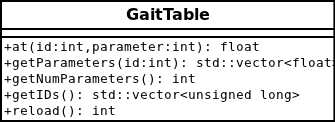
\includegraphics[width=0.3\textwidth]{images/Class_diagram_GaitTable_members.png}
        \caption{GaitTable class diagram}\label{fig:software_class_gaittable_class}
\end{figure}

The class \emph{GaitTable} stores the oscillator parameters relating them to a ID. The data is stored as a table, with the different parameters for each ID stored as rows of the table. An example of the internal representation of a gait table for the main oscillator parameters is shown in table \ref{table:gait_table_example}. 

\begin{table}[h]
\centering
\begin{tabular}{|c||c|c|c|} \hline
 ID & Amplitude & Offset & Phase \\ \hline \hline
83506 & 60 & 0 & 0 \\ \hline
78896 & 60 & 0 & 120 \\ \hline 
\end{tabular}
\caption{Example of the internal contents of a gait table for a 2 module configuration}
\label{table:gait_table_example}
\end{table}

The \emph{GaitTable} can receive queries for a given ID, and then it returns all the parameters corresponding to that ID. The data is stored and read using text files, in a format that is compatible with the Matlab/Octave text file format.\\

\subsection{Class Orientation}
\label{software_class_orientation}


\begin{figure}[h]
		\centering
        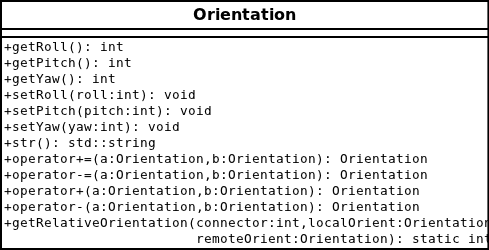
\includegraphics[width=0.45\textwidth]{images/Class_diagram_Orientation.png}
        \caption{Orientation class diagram}\label{fig:software_class_orientation_class}
\end{figure}

For calculating the ID based on the position of the module inside the modular robot, a module needs to know the relative orientation between the attached connectors. To work with those Orientations, the class \emph{Orientation} was implemented. \emph{Orientation} is supposed to be measured by the module with a Inertial Measuremente Unit (IMU) but, as the modules do not have a IMU because of hardware limitations, the IMU is currently simulated by reading the initial values that the IMU would return from the robot configuration file.\\

For expressing the orientation, we are using Tait-Bryan angles, a representation largely used in aeronautics, and the one that the IMU returns by default. This representation, similar to the Euler Angles, expresses the orientation of an object with three angles: roll, pitch and yaw. These angles represent rotations around the three main axes of a fixed reference frame, roll corresponding to the rotation around the Z axis; pitch being a rotation about the Y axis and finally yaw, a rotation about the X axis. Notice that, unlike Euler Angles, these rotations are performed around a reference frame that is fixed in the world, not in the object, and therefore it does not rotate with the object.\\
\begin{figure}[h]
		\centering
        \begin{subfigure}[b]{0.4\textwidth}
                \centering
                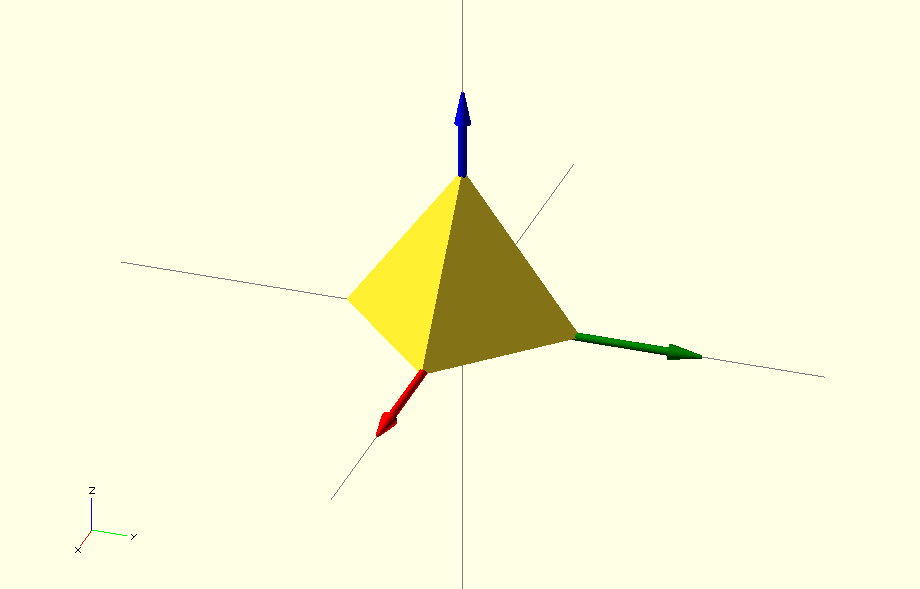
\includegraphics[width=\textwidth]{images/Orientation/tait-bryan-01.png}
                \caption{Initial orientation}
                \label{fig:soft_orientation_initial}
        \end{subfigure}
        ~
        \begin{subfigure}[b]{0.4\textwidth}
                \centering
                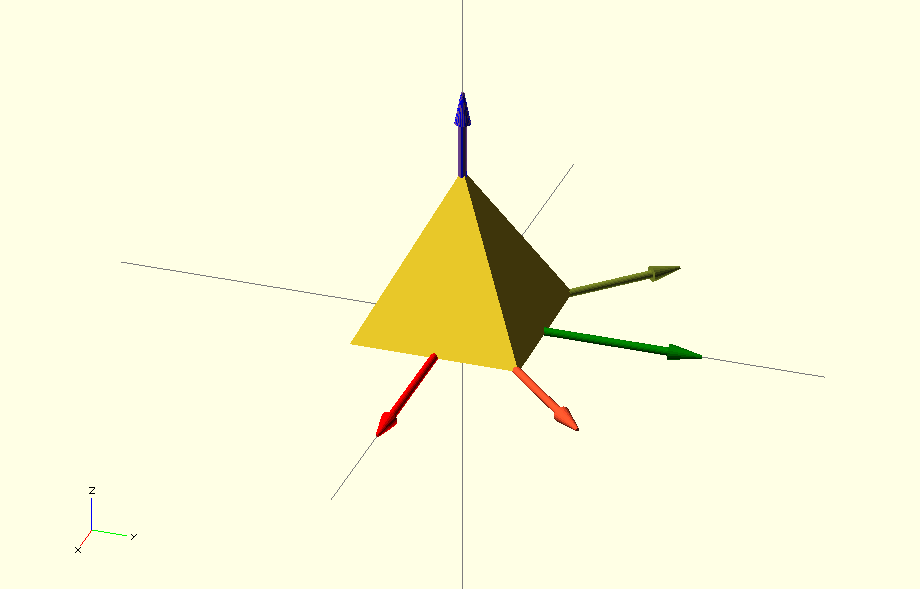
\includegraphics[width=\textwidth]{images/Orientation/tait-bryan-02.png}
                \caption{Roll 45º around Z axis }
                \label{fig:soft_orientation_roll}
        \end{subfigure}
        ~
        \begin{subfigure}[b]{0.4\textwidth}
         	   \centering
                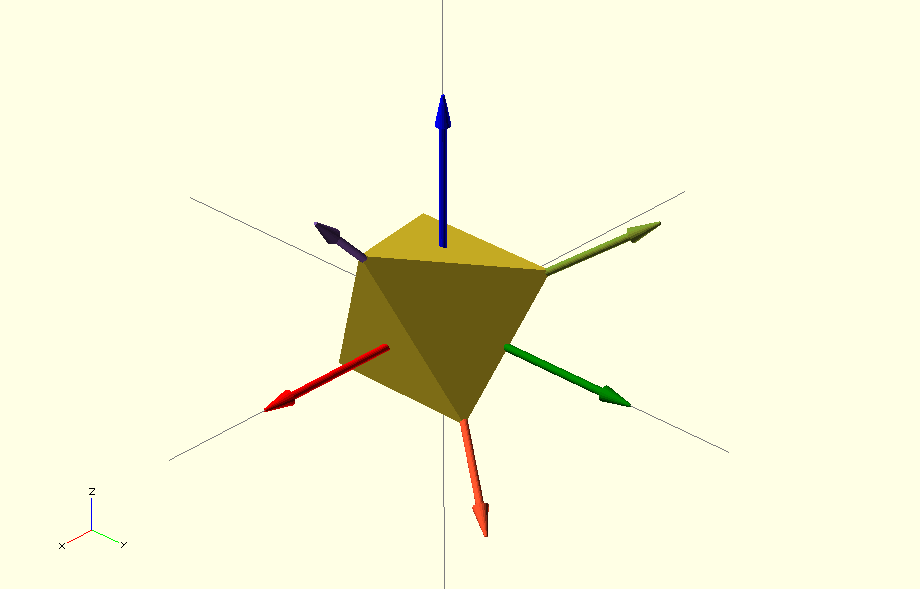
\includegraphics[width=\textwidth]{images/Orientation/tait-bryan-03.png}
                \caption{Pitch 45º around Y axis}
                \label{fig:soft_orientation_pitch}
        \end{subfigure}        
        ~
        \begin{subfigure}[b]{0.4\textwidth}
         	   \centering
                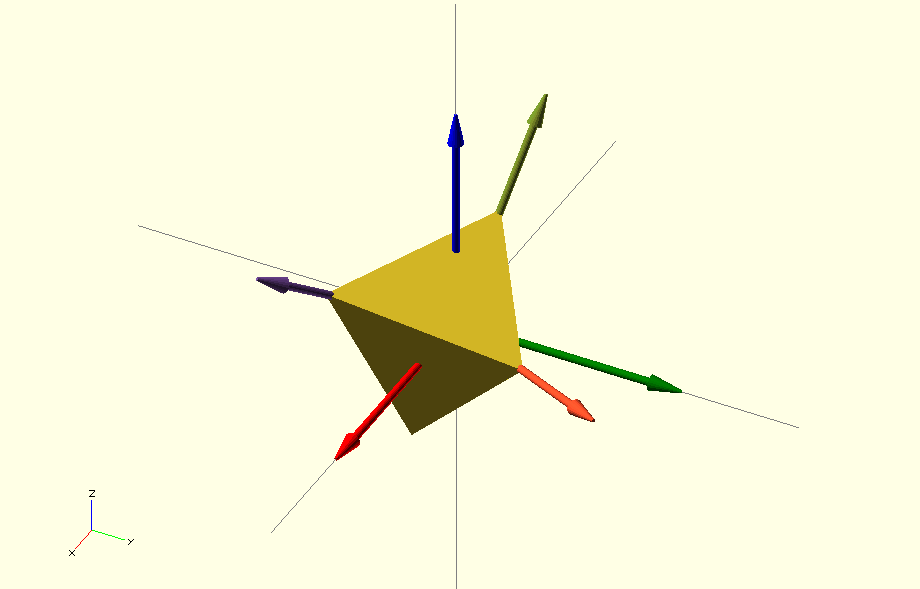
\includegraphics[width=\textwidth]{images/Orientation/tait-bryan-04.png}
                \caption{Yaw 45º around X axis}
                \label{fig:soft_orientation_yaw}
        \end{subfigure}
        \caption{Steps to obtain a pyramid with a orientation of (45º, 45º, 45º) expressed in Tait-Brian angles RPY}\label{fig:soft_orientation_example}
\end{figure}


Inside the \emph{Orientation} class, angles are bound to the interval [0, 360), and the class counts with several functions to perform simple arithmetic operations with them, as well as to convert them to a string for storing the \emph{Orientation} on the data field of the \emph{Hormone} class. For calculating the relative rotation between two modules, the function \emph{getRelativeOrientation} can be used, passing it the ID of the connector that is used as reference (0, 1, 2 and 3 for front, right, back and left, respectively) as well as the local and remote module orientations.\\

The relative rotation between two modules is expressed as an integer value from 0 to 3 that represents the number of 90º steps we have to rotate the local module around the axis of the local reference system that is in the same direction as the normal vector of the local connector surface, such as the Z axis of the local reference system of both modules coincide. This is explained in more detail, with graphical examples in section \ref{config_repy_description}.\\

The algorithm used by \emph{getRelativeOrientation()} to calculate the relative rotation value is the following:

\begin{enumerate}
	 \item Roll, pitch and yaw angles are equivalent to Euler XYZ angles, so we use this property to calculate the transformation matrices for both reference systems (the one from the local module and the one from the remote module) by multiplying the rotation matrices around X (yaw), Y (pitch) and Z (roll).
	 \[ ^{0}H_A = Rot_X(\gamma_A) * Rot_Y(\beta_A) * Rot_Z(\alpha_A) \]
	 \[ ^{0}H_B = Rot_X(\gamma_B) * Rot_Y(\beta_B) * Rot_Z(\alpha_B) \]
	 
	 Were $~^{0}H_{x}$ is the homogeneous transformation matrix to go from the absolute reference system to x, A is the local module reference system, B is the remote module reference system and $\alpha$, $\beta$ and $\gamma$ are roll, pitch and yaw angles, respectively. In a matricial form, the previous equations become:
	 
	 \[  ^{0}H_A =  
	 \begin{bmatrix}
	 1 & 0 & 0 \\ 
	 0 & \cos(\gamma_A) & -\sin(\gamma_A)\\
	 0 & \sin(\gamma_A) & \cos(\gamma_A)
	 \end{bmatrix}
	 \begin{bmatrix}
	 \cos(\beta_A)  & 0 & \sin(\beta_A) \\ 
	 			0   & 1 & 			0  \\
	 -\sin(\beta_A) & 0 & \cos(\beta_A)
	 \end{bmatrix}
	 	 \begin{bmatrix}
	  \cos(\alpha_A)  & -\sin(\alpha_A) & 0 \\ 
	  \sin(\alpha_A)  &  \cos(\alpha_A) & 0 \\
	 			   0  &               0 & 1
	 \end{bmatrix}\]	 	 
	 \[  ^{0}H_B =  
	 \begin{bmatrix}
	 1 & 0 & 0 \\ 
	 0 & \cos(\gamma_B) & -\sin(\gamma_B)\\
	 0 & \sin(\gamma_B) & \cos(\gamma_B)
	 \end{bmatrix}
	 \begin{bmatrix}
	 \cos(\beta_B)  & 0 & \sin(\beta_B) \\ 
	 			0   & 1 & 			0  \\
	 -\sin(\beta_B) & 0 & \cos(\beta_B)
	 \end{bmatrix}
	 	 \begin{bmatrix}
	  \cos(\alpha_B)  & -\sin(\alpha_B) & 0 \\ 
	  \sin(\alpha_B)  &  \cos(\alpha_B) & 0 \\
	 			   0  &               0 & 1
	 \end{bmatrix}\]\\
	 
	 \item We undo the rotation of the local module reference system to make it coincide with the absolute reference frame, and apply the same inverse transformation to the remote module reference system, obtaining the homogeneous tranformation matrix to go from A (local module) to B (remote module):
	 \[  ^{A}H_B = ~^{A}H_0 \cdot ~^{0}H_B = (~^{A}H_0)^{-1} \cdot ~^{0}H_B  \]
	 
	 \item We find the Z vector of the remote reference system ($ \vec{k'}$) by multiplying the unit Z vector of the absolute reference system ($ \vec{k}$) by the homogeneous tranformation matrix.
	 \[ \vec{k'} = ~^{A}H_B ~ \vec{k} = ~^{A}H_B \begin{bmatrix} 0\\ 0\\ 1 \end{bmatrix}\]
	 
	 \item Iteratively, the vector $\vec{k}$ is rotated in steps of 90º until it matches with the vector $\vec{k'}$ calculated in the previous step. The axis of rotation depends on which is the connector of the local module being evaluated, for the front and back connectors, the Y axis is used, whereas for the left and right connectors, it is the X axis. The number of steps required to match them is the relative rotation value returned by the function.
\end{enumerate}


%%%%%%%% EXECUTABLES %%%%%%%%%%%%%%%%%%%%%%%%%%%%%%%%%%%%%%%%%%%%%%%%%%%%%%%%%%
\section{Applications}
\label{software_apps}

Apart from the main framework, the Hormodular software has several applications to perform the optimization of the locomotion parameters and their evaluation either on the simulated robot, or the real robot via serial port. The source code for these applications can be found in the ``src/apps'' folder inside the project main directory and, once compiled, these applications can be found in the ``bin'' folder.

\subsection{evolve-gaits}
\label{software_evolve-gaits}
The program ``evolve-gaits'' is used for finding the best oscillator parameters in order to achieve an optimal gait on a given modular robot configuration. This program uses the Evolutionary Computing Framework (ECF) library to perform the optimization of those parameters using the Differential Evolution algorithm (Described on section \ref{evolution_algorithm}). For the evaluation of the gait generated by the oscillator parameters of an individual of the Differential Evolution population we implemented a very simple controller that just performs the joint position update according to the joint values provided by the sinusoidal oscillators with the parameters to be evaluated.\\

The usage of the program is not complex, as it only takes an argument for its execution, the evolution configuration file. The configuration file is a xml file containing a set of tags defined by the authors of the ECF library in order to configure the optimization algorithm. Some of the parameters that can be configured with this file are: the type of optimization algorithm and its parameters, the type of genotype to be used, the population size and the number of iterations, among others. ECF also allows the users of the library to define custom tags to configure other aspects of the evolution, such as the path of the robot configuration file, the evaluation time of the robot gait, or the limits of the sinusoidal oscillator parameters.\\

The program will read this parameters and it will execute the optimization algorithm. A log file is configured to be automatically created to track the progress of the algorithm, and a milestone file is generated with data that can be used to resume the execution of the evolution in case the program crashes or is interrupted. This milestone file also contains the genotype of the best individual, from we will extract the oscillator parameters for the best gait.\\

These parameters are encoded in the genotype with normalized values in the interval $[-1, 1]$ due to limitations of the ECF that do not allow to set different value limits for different parameters of a single genotype. To obtain the non-normalized values without doing operations by hand, and set them on a gait table, a Octave/Matlab simple script was developed, and can be found in the ``Utils'' folder that will generate the required data from the normalized values returned by the evolution program.\\


\subsection{evaluate-gaits-sim}
\label{software_evaluate-gaits-sim}
Once the best parameters have been found, we would want to evaluate those parameters, as well as the hormone communication protocol, in order to check if a suitable gait was found, and if the hormone controller performs as desired. In order to test it on the simulated robot, the ``evaluate-gaits-sim'' application can be used.\\

This program just creates a \emph{ModularRobot} instance with a simulated \emph{ModularRobotInterface} and configures it with the parameters specified by the user. Then, it runs the simulation for the specified run time and reports the results of the evaluation to the user. The resulting gaits can be observed on the simulation viwer offered by OpenRAVE.\\

The usage of this program is simple. It requires the user to call the program specifying the xml robot configuration file and the time the robot will be simulated (simulation time), with an optional parameter being the simulation step time, which  is 0.25 ms by default. At the end of the evaluation, the program shows the real time that it took to simulate the robot during the run time specified by the user, as well as the distance travelled by the robot.\\


\subsection{evaluate-gaits-serial}
\label{software_evaluate-gaits-serial}
Since the final objective is to control a real modular robot with the controller, it is very useful to test the gaits and the hormone controller on the real modular robot. For that purpose the ``evaluate-gaits-serial'' program exists.\\

This program creates a \emph{ModularRobot} with a \emph{SerialModularRobotInterface}, connecting with the robot through the serial port and sending it the commands required to drive the servos to the desired positions. The modular robot, in the current state of development acts as a ``dummy'' robot: the distributed controller for each of the modules runs on the computer, and it sends to the robot the position of the different joints, which allows the robot to move, and allow us to test if the gaits are effective and optimal in a real-world environment.\\

The parameters for running the ``evaluate-gaits-serial'' program are exactly the same as the ones for the simulated robot evaluation, but in this case the step time corresponds to the rate of update of the robot joints, which has been increased to 2 ms by default due to bandwidth limitations of the serial port.\\


\subsection{Utils}
\label{software_utils}

Apart from the main programs, the repository includes a series of scripts that solve in a fast way some of the repetitive and dull tasks that appear during the development process.\\

The first one is a Python script called \emph{IDcalculator.py}, that takes a string containing the connection description in a human-readable way as argument and translates it to the actual ID number. An example of its usage would be:
\Bash
\begin{lstlisting}
  $ python IDcalculator.py "((L,90), X, (R, 270), X)"
\end{lstlisting}
%$

In which each of the four elements of the top level 4-tuple is the information of the remote connector connected to the front, left, right and back connector, respectively, with `X' denoting that there is nothing connected to that connector. The elements of the inner tuples are the remote connector attached to the local connector, and coded with the initial of that connector (i.e. L for left or R for right) and the relative orientation between connectors. In the example above, that ID would correspond to a module with the left connector of another module attached to the front connector at an relative angle of 90º, and the right connector of other module attached to the back connector at a relative angle of 270º which corresponds to the ID 82644.\\

The second one is a Octave/Matlab script called \emph{vectorToTable.m} that converts a vector containing the genotype resultant from the optimization process to a gait table. This genotype contains the optimized oscillator parameters normalized in the interval $[-1,1]$. The parameter limits are specified when calling the function defined in the script, returning a table with the parameters already scaled back to the non-normalized form. If we want to obtain the gait table for a \emph{MultiDof-9-tripod} configuration, optimized with $A_{max} = 80º$,  $O_{max} = 45º$, $\phi_{max} = 360º$ and $f_{max} = 1.5Hz$, the function would be called as follows:

\Bash
\begin{lstlisting}
  $ octave
  
  octave:1> v = [ 0.434181, 0.845216, 0.470191, -0.846046, 0.790331, -0.264226, 0.857843, -0.527548, -0.67852, 
  0.917075, -0.306737, 0.164061, 0.190244, -0.522919, -0.411536, -0.44878, -0.689907, 0.402322, 0.159478,
  -0.348137, 0.579257, 0.0460117];
  
  octave:2> vectorToTable( v, 7, 80, 45, 360, 1.5, 1);
\end{lstlisting}
%$

This will generate two files: the gait table of the main oscillator parameters ( $A$, $O$, $\phi$), called \emph{Tx.txt} and the gait table containing the frequency, named \emph{fx.txt}, where `x' is the configuration ID in both cases.


%%%%%%%% COMPILE & RUN %%%%%%%%%%%%%%%%%%%%%%%%%%%%%%%%%%%%%%%%%%%%%%%%%%%%%%%%%%
\section{Compiling \& running Hormodular}
\label{software_compile}

The source code of the \emph{Hormodular} framework is releashed under a open source GPLv3 license, allowing any researcher interested in modular robotics to use this code, study it, improve it and publish their modified version, with a compulsory attribution to the original author. This way the results presented in this work can be evaluated and tested by other researches, reproducing the experiments with the same software to test their validity.\\

Following the open source approach, the project has been developed using open source software under a GNU/Linux system. Therefore, the code is only tested on the GNU/Linux platform and there are no guarantees that it works on other platforms suchs as Windows or Mac.\\

This section explains how to install the required dependencies required by \emph{Hormodular}, as well as how to download and compile the source code, and how to run it.

\subsection{Installing dependencies}
\label{software_install_dependencies}

\subsubsection{Installing CMake}
\label{software_install_cmake}
CMake is an open source cross-platform program that automates the compilation and installation of software by generating the corresponding makefiles and environment to be used with the compiler desired by the user. CMake can be found in the repositories of many GNU/Linux distributions, or downloaded from \url{http://www.cmake.org/cmake/resources/software.html} , either already compiled or as source code.\\

To be installed from the GNU/Linux terminal on a Ubuntu system, the following command can be used:
\Bash
\begin{lstlisting}
  $ sudo apt-get install cmake
\end{lstlisting}
%$


\subsubsection{Installing OpenRAVE}
\label{software_install_openrave}

OpenRAVE is the open source simulation library chosen to simulate the modular robot and evaluate its locomotion gaits for the different configurations.\\

Detailed instructions for installing OpenRAVE can be found on their website: \url{http://openrave.org/docs/latest_stable/install/}. On a GNU/Linux, Ubuntu-based system, the commands for installing OpenRAVE from the repository are:

\newpage

\Bash
\begin{lstlisting}
  $ sudo add-apt-repository ppa:openrave/release
  $ sudo apt-get update
  $ sudo apt-get install openrave
\end{lstlisting}
%$

If these commands do not work, or if it is preferred, OpenRAVE can be installed from the sources, following the instructions that can be found in: \url{http://openrave.org/docs/latest_stable/coreapihtml/installation.html}\\

\subsubsection{Installing OpenMR plugin for OpenRAVE}
\label{software_install_openmr}

The OpenMR plugin for OpenRAVE adds the servocontroller to the controllers available by default on OpenRAVE. As well as the 3D models for simulating REPY and REPY-2.0 based modular robots. It was originally developed by Juan Gonzalez-Gomez but his version is no longer maintained, so we recommend to download it from our repository: \url{https://github.com/David-Estevez/openmr}.\\

The code is ready to be compiled using CMake. In a GNU/Linux terminal, the commands to install it would be (it is assumed that the user is already in the openMR project folder):
\Bash
\begin{lstlisting}
  $ mkdir build
  $ cd build
  $ cmake ..
  $ make
  $ sudo make install
\end{lstlisting}
%$

\subsubsection{Installing the Evolutionary Computing Framework}
\label{software_install_ecf}

The Evolutionary Computing Framework provides the optimization algorithms required to obtain the sinusoidal oscillator parameters necessary to achieve an optimal locomotion gait. All the information related to the ECF can be found on its website: \url{http://gp.zemris.fer.hr/ecf/}.\\

In order to install the ECF, it is required to download the source code, whose link can be found in their website, under the ``Download'' section. Instructions for building the ECF can be found in: \url{http://gp.zemris.fer.hr/ecf/install.html}, but for a GNU/Linux system they can be summarized on running the following commands on the source code directory:
\Bash
\begin{lstlisting}
  $ ./configure
  $ make
  $ sudo make install
\end{lstlisting}
%$

In case this procedure fails for any reason, a script (\emph{ecf\_install.sh}) is provided for a semi-automatic installation.

\subsubsection{Installing TinyXML2}
\label{software_install_TinyXML2}

TinyXML2 is a lightweight library required for parsing the robot configuration XML files. The source code can be downloaded from their git repository: \url{https://github.com/leethomason/tinyxml2} either as a zip file or, if git is installed, with the following command:
\Bash
\begin{lstlisting}
  $ git clone https://github.com/leethomason/tinyxml2
\end{lstlisting}
%$\\

Once the source code is downloaded, it can be build and installed using CMake:
\Bash
\begin{lstlisting}
  $ mkdir build
  $ cd build
  $ cmake ..
  $ make
  $ sudo make install
\end{lstlisting}
%$

\subsubsection{Installing Eigen}
\label{software_install_eigen}

Eigen is an open source library for making linear algebra operations. It is used to calculate the relative rotation between two modules from their Tait-Bryan angles. Eigen is a C++ template library, so no code has to be compiled for its installation, copying the headers to the system libraries folder is enough.\\

If Eigen is available on the repositories, it can be installed with the following command:
\Bash
\begin{lstlisting}
  $ sudo apt-get install libeigen3-dev
\end{lstlisting}
%$\\

Otherwise, the source code can be downloaded from their webpage: \url{http://eigen.tuxfamily.org/index.php?title=Main_Page} , and installed using CMake:
\Bash
\begin{lstlisting}
  $ mkdir build
  $ cd build
  $ cmake ..
  $ sudo make install
\end{lstlisting}


\subsection{Building Hormodular}
\label{software_install_hormodular}

After all the different depencies have been installed, the source code of Hormodular can be downloaded from our repository: \url{https://github.com/David-Estevez/hormodular} , either as a zip file or with the following command, if git is installed:
\Bash
\begin{lstlisting}
  $ git clone https://github.com/David-Estevez/hormodular
\end{lstlisting}
%$\\

Once the code is downloaded, the procedure to build the project using CMake is simple:\Bash
\begin{lstlisting}
  $ mkdir build
  $ cd build
  $ cmake ..
  $ make
  $ sudo make install
\end{lstlisting}
%$

\subsection{Running Hormodular}
\label{software_run_hormodular}

Once compiled, the different applications should appear on the ``bin'' folder, ready to be executed. The purpose of each of the applications is explained in section \ref{software_apps}.